\documentclass[a4paper,12pt]{book}

\usepackage{url}
\usepackage[brazil]{babel}
\usepackage[pdftex]{graphicx}
\usepackage[pdftex]{hyperref}

\title{Xadrez em Realidade Aumentada - Manual}
\author{
		Douglas Bettioli Barreto (NUSP 6920223)
		\and Giancarlo Rigo (NUSP 6910034)
		\and Rafael Reggiani Manzo (NUSP 6797150)
	   }

\begin{document}

\maketitle

\part{Manual do usu\'ario}
\label{part:manualdousuario}

\part{Manual do Desenvolvedor}
\label{part:manualdodesenvolvedor}
	\chapter{Diagrama de classes}
	\label{ch:diagramadeclasses}
	\begin{figure}[h]
	\centering
	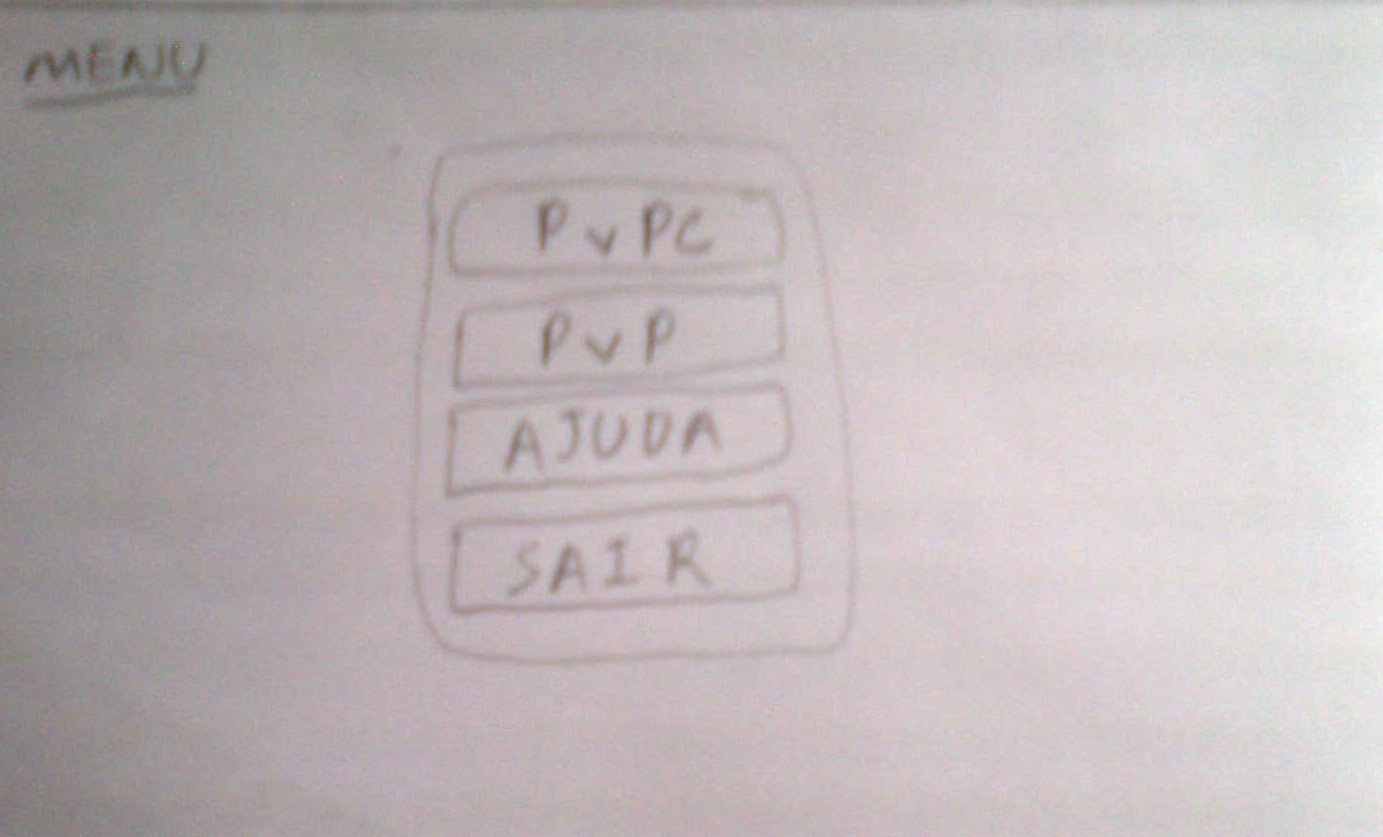
\includegraphics[width=0.7\textwidth]{menu}
	\end{figure}
	
	\chapter{Prova de conceito}
	\label{ch:provadeconceito}
		\section{Introdu\c c\~ao}
		\label{sec:pcintroducao}
		A prova de conceito consistiu em abordar os pontos chave do projeto no que se
		refere a realidade aumentada. Nela, foram tratados temas como o reconhecimento
		de multiplos marcadores e a capacidade de obter as coordenadas do marcador no
		espa\c co.
		
		\section{Pacote AugmentedReality}
		\label{sec:pcpacoteaugmentedreality}
		
		No momento, este pacote possui as classes ARObject e AROperation. Mas, com o
		desenvolvimento do projeto, devem ser criadas novas classes.

		
\end{document}
